\section{Feedback systems}

The transfer function of a feedback system can be derived from its block diagram as follows:
\begin{figure}[H]
    \centering
    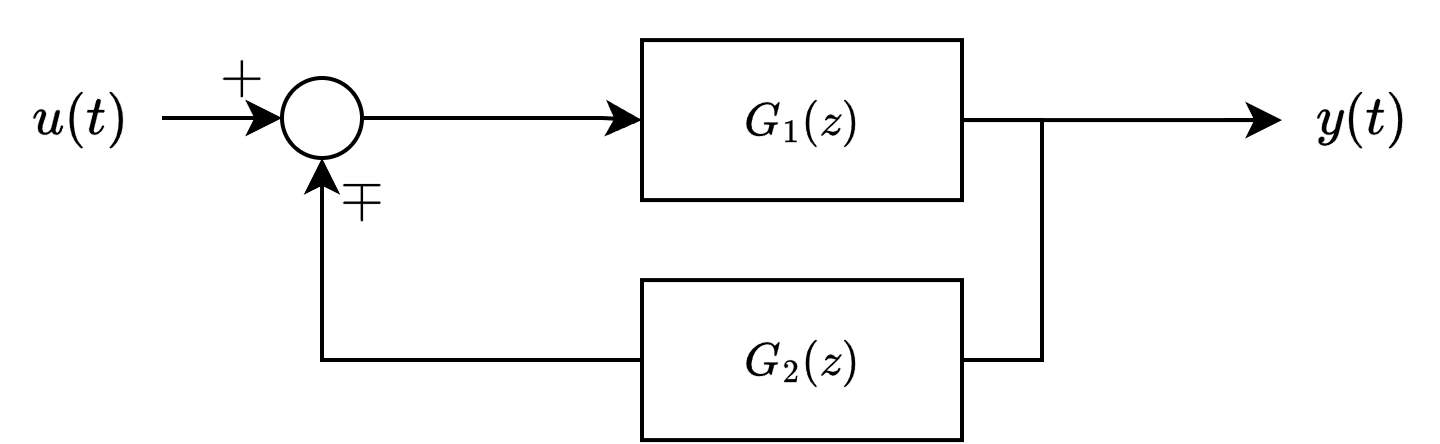
\includegraphics[width=0.6\linewidth]{images/feedback.png}
\end{figure}
We can write the equation for the output $y(t)$ in terms of the input $u(t)$ and the transfer functions $G_1(z)$ and $G_2(z)$:
\begin{align*}
    &y(t)=G_1(z)\left(u(t)\pm G_2(t)y(t)\right) \rightarrow \\
    &y(t)\left(1 \pm G_1(z)G_2(z)\right)=G_1(z)u(t) \rightarrow \\
    &y(t)=\dfrac{G_1(z)}{1 \pm G_1(z)G_2(z)}u(t)
\end{align*}
This formula represents the general transfer function for any feedback system. 
It shows that the input-output behavior of the closed-loop system is relatively straightforward, as many dynamics are hidden in the non-observable part of the system by design. 

\subsection{Feedback system stability}
To check the stability of a feedback system, we create the loop function $L(z)$ defined as the product of the transfer functions $G_1(z)$ and $G_2(z)$:
\[L(z)=G_1(z)\cdot G_2(z)\]
From this loop function, we can construct the characteristic polynomial $\chi(z)$ by considering its numerator and denominator:
\[\chi(z)=L_{N}(z)\pm L_D(z)\]
Here, $L_{N}(z)$ represents the numerator of the closed-loop function, and $L_{D}(z)$ represents the denominator.
\begin{theorem}
    The feedback system is asymptotically stable if and only if all the roots of the characteristic polynomial $\chi(z)$ are strictly inside the unit circle.
\end{theorem}
In summary, to determine the stability of a feedback system, we analyze the roots of the characteristic polynomial obtained from the loop function $L(z)$. 
If all the roots lie inside the unit circle in the complex plane, the system is asymptotically stable. 
Otherwise, if any root lies on or outside the unit circle, the system is unstable.